\section{Box Class Reference}
\label{classBox}\index{Box@{Box}}
{\tt \#include $<$box.h$>$}

Inheritance diagram for Box::\begin{figure}[H]
\begin{center}
\leavevmode
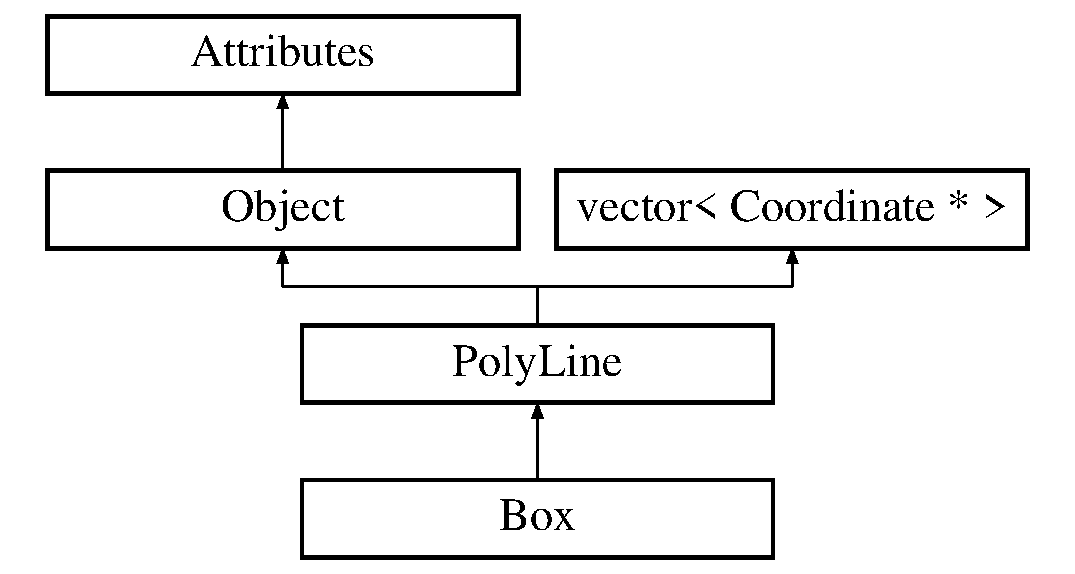
\includegraphics[height=4cm]{classBox}
\end{center}
\end{figure}
\subsection*{Public Methods}
\begin{CompactItemize}
\item 
{\bf Box} ()
\item 
{\bf Box} ({\bf Coordinate} $\ast$coordinate1, {\bf Coordinate} $\ast$coordinate2)
\item 
{\bf $\sim$Box} ()
\end{CompactItemize}


\subsection{Detailed Description}
This class handles box objects. This class is derived from {\bf Poly\-Line} {\rm (p.\,\pageref{classPolyLine})}. \begin{Desc}
\item[Author: ]\par
Anthony Liekens \end{Desc}




\subsection{Constructor \& Destructor Documentation}
\index{Box@{Box}!Box@{Box}}
\index{Box@{Box}!Box@{Box}}
\subsubsection{\setlength{\rightskip}{0pt plus 5cm}Box::Box ()}\label{classBox_a0}


Constructor. Constructs a box object. \index{Box@{Box}!Box@{Box}}
\index{Box@{Box}!Box@{Box}}
\subsubsection{\setlength{\rightskip}{0pt plus 5cm}Box::Box ({\bf Coordinate} $\ast$ {\em coordinate1}, {\bf Coordinate} $\ast$ {\em coordinate2})}\label{classBox_a1}


Constructor. Constructs a box object. \begin{Desc}
\item[Parameters: ]\par
\begin{description}
\item[{\em 
coordinate1}]One corner of the box \item[{\em 
coordinate2}]Opposite corner of the box \end{description}
\end{Desc}
\index{Box@{Box}!~Box@{$\sim$Box}}
\index{~Box@{$\sim$Box}!Box@{Box}}
\subsubsection{\setlength{\rightskip}{0pt plus 5cm}Box::$\sim$Box ()}\label{classBox_a2}


Destructor. Destructs a box object. 

The documentation for this class was generated from the following files:\begin{CompactItemize}
\item 
{\bf box.h}\item 
{\bf box.cpp}\end{CompactItemize}
